
%%%%%%%%%%%%%%%%%%%%%%%%%%%%%%%%%%%%%%%%%%%%%%%%%%%%%%%%%%%%%%%%%%%%%%%%%%%%%%%%%%%%%%%%%%%%%%
\chapter{3D Lattice-Boltzmann Models of the Complete Conjugate Heat Transfer of Helium Purge Gas and Ceramic Pebble Beds}\label{sec:lbm-studies}

In this section I apply the relatively new techniques of lattice-Boltzmann method (LBM) numerical modeling to study the complete interstitial flow of helium through a packed bed of lithium ceramics. A discussion on the development of the LBM method was given in \Cref{sec:modeling-lbm}. In that section, the advantages of LBM for porous flow simulations were made apparent, namely the potential for extreme parallelization due to the highly local calculations on lattice nodes as well as the straightforward implementation of boundary conditions for the complex geometry of porous networks.

For the implementation of DEM and LBM coupling, pebble packing structures are generated with DEM simulations then mapped into the LBM nodal grids where the thermofluid and conjugate heat transfer models solve momentum and thermal conservation equations. The DEM-LBM approach is a one-way coupled approach in that LBM results are not currently fed back into DEM simulations for future packing evolution. The sacrifice of two-way coupling (that is present in the volume-averaged CFD-DEM model) offers instead to understand the tortuous helium flow and its impact on thermal transport in the tritium breeding ceramic pebble beds.

The first part of this section will discuss the process of determining certain numerical techniques needed in mapping DEM data into LBM nodes. Once the characteristics of the pebble bed parameters are understood, sample models of pebble beds from \Cref{sec:isfnt-12} are loaded into the DEM-LBM solver and analyzed.


\section{DEM Mapping and Lattice Parameters}
In the process of mapping DEM data into LBM nodes, several computational choices must be made. The first is the resolution of the LBM lattice. That is, how many lattice nodes per pebble diameter are desired. The resolution will ultimately determine the size of the lattice spacing and lattice time step. The larger the resolution, the smaller the step size and smaller the time step. The second choice relates to digitalizing the DEM `sphere' into a discretized lattice. When a pebble of radius $R_p$ is mapped onto a lattice with discrete steps, the size of the sphere is over-represented and the LBM lattice does not faithfully reproduce the correct void fraction from DEM.

\begin{figure}[h]
        \centering
        \begin{subfigure}[b]{0.2\textwidth}
                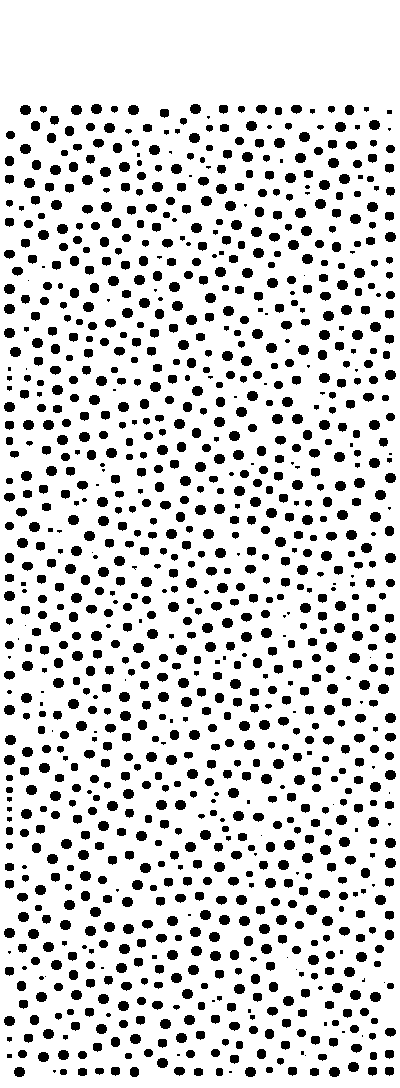
\includegraphics[width=\textwidth]{figures/lbm/2d-res20-k050.png}
                \caption{$\phi = 0.181$ in pebble bed section with $k = 0.50$.}
                \label{fig:2d-res20-k050}
        \end{subfigure}%
        ~
        \begin{subfigure}[b]{0.2\textwidth}
                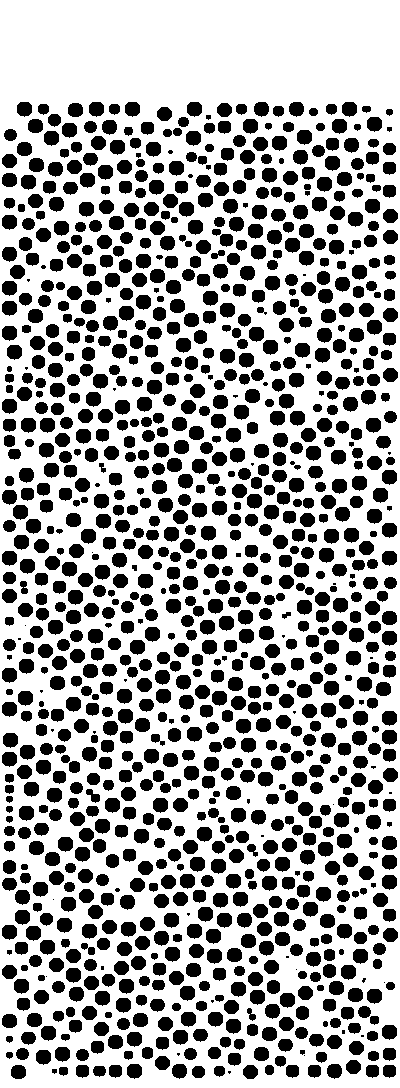
\includegraphics[width=\textwidth]{figures/lbm/2d-res20-k075.png}
                \caption{$\phi = 0.389$ in pebble bed section with $k = 0.75$.}
                \label{fig:2d-res20-k075}
        \end{subfigure}%
        ~
          %add desired spacing between images, e. g. ~, \quad, \qquad, \hfill etc.
          %(or a blank line to force the subfigure onto a new line)
        \begin{subfigure}[b]{0.2\textwidth}
                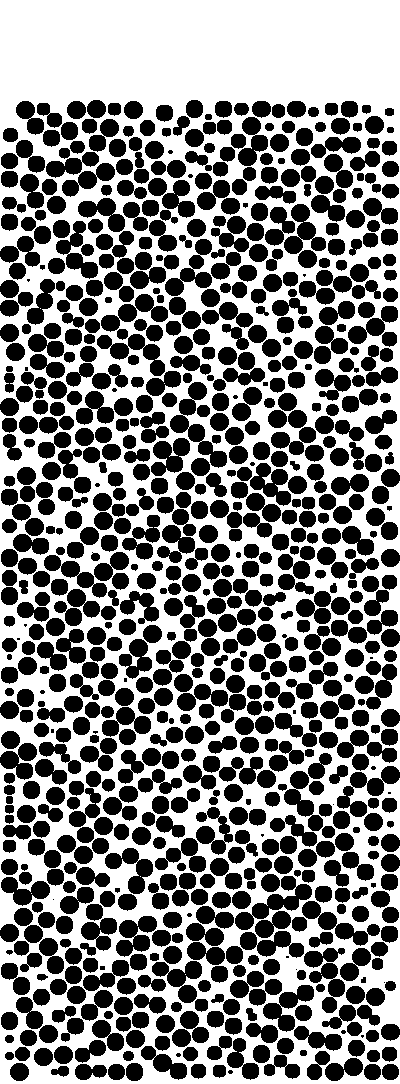
\includegraphics[width=\textwidth]{figures/lbm/2d-res20-k090.png}
                \caption{$\phi = 0.555$ in pebble bed section with $k = 0.90$.}
                \label{fig:2d-res20-k090}
        \end{subfigure}
        ~
        \begin{subfigure}[b]{0.2\textwidth}
                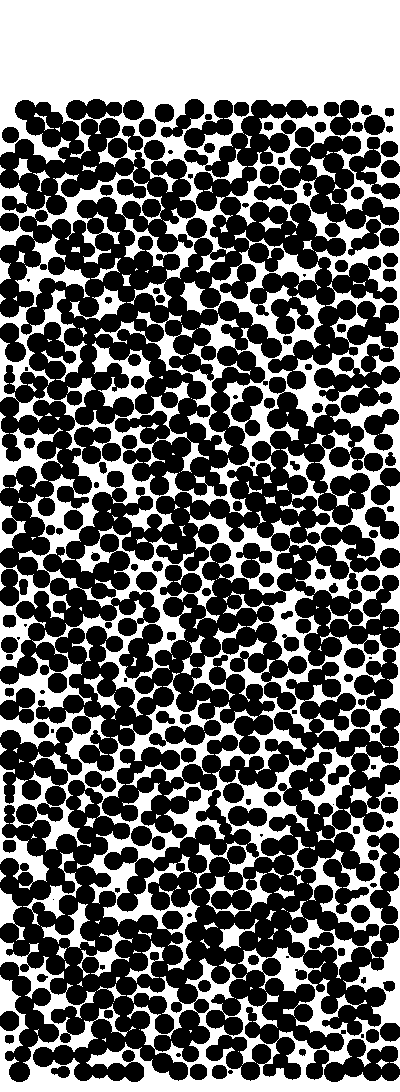
\includegraphics[width=\textwidth]{figures/lbm/2d-res20-k100.png}
                \caption{$\phi = 0.667$ in pebble bed section with $k = 1.00$.}
                \label{fig:2d-res20-k100}
        \end{subfigure}
        \caption{For a given resolution, the scaling parameter $k$ will result in different packing fractions. These mappings were generated from a pebble bed with $\phi =0.64$; only a specific $k$ will yield that void fraction after mapping into LBM.}\label{fig:2d-dem-lbm-mapping}
\end{figure}

Before attempting to handle a full-scale pebble bed from DEM, we begin with a two-dimensional lattice of a representative pebble bed. In the first step, we choose a resolution of $\res=20$ and then vary a radius-drawing-parameter, $k$. This parameter simply states that when a DEM pebble is mapped into an LBM lattice, that the radius is scaled by this value before mapping. To highlight the effects of $k$, some example two-dimensional lattices are shown in \Cref{fig:2d-dem-lbm-mapping}. The two-dimensional lattice is loaded from the $\phi =0.64$ initial packing of \Cref{sec:isfnt-12}.

\begin{figure}[h]
    \centering
    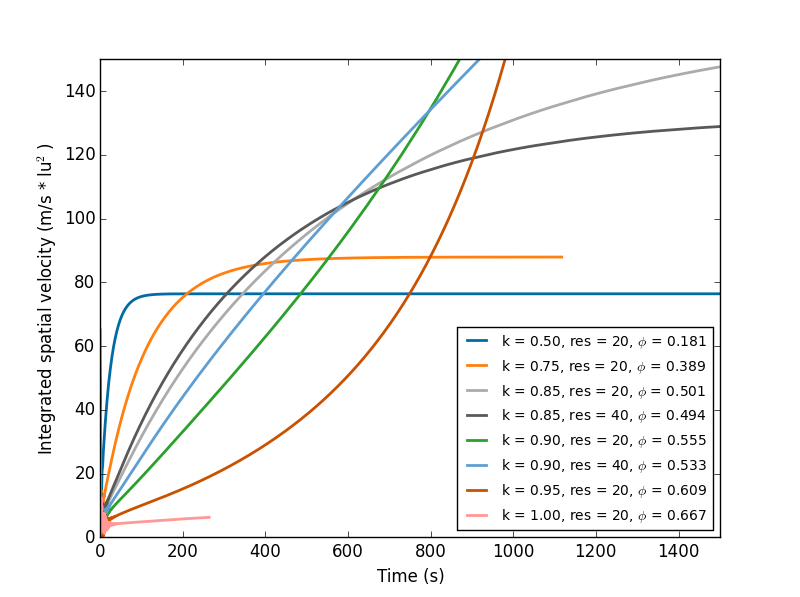
\includegraphics[width=0.75\textwidth]{figures/lbm/2d-lbm-settings-velocity}
    \caption{Integrated system velocity shows stable lattice configurations in two dimensions.}\label{fig:2d-lbm-settings-velocity}
\end{figure}

Other lattices were generated with varying values of $k$ and $\res$. Using simple boundary conditions of no-slip on the left and right walls, a Neumann boundary condition at the outlet (top) and constant velocity at the inlet (bottom), all latices were tested to find the stability of the resolutions and packings. To determine if a steady-state condition was reached, the velocity of the entire lattice was integrated. The value has units of $\psi = [m/s][lu^2]$, with dimensionless lattice spacing units. The value of $\psi$ is plotted in \Cref{fig:2d-lbm-settings-velocity}. From \Cref{fig:2d-lbm-settings-velocity}, we see a steady-state velocity is reached in all of the low-packing fraction lattices. As the packing fraction increased, following the increase of $k$, we see the system velocity slowly become unstable. When $k$ = 0.9, with a packing fraction of $\phi = 0.555$, the system approximately linearly increases into unstable values. Note, for the case when $k=1$, the density calculated in this system blew up to $\infty$ in less than 300 steps, so the velocity profile does not have a chance to demonstrate the unstable increase. For that bed, the packing fraction was high enough that there was not a continuous path available between inlet and outlet.

\begin{figure}[h]
    \centering
    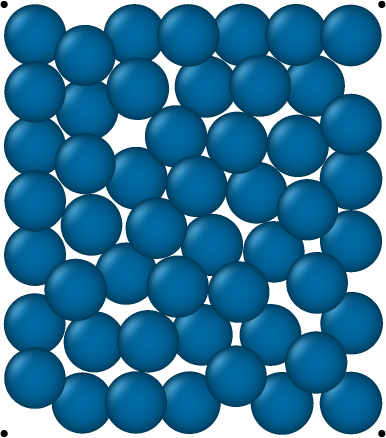
\includegraphics[width=0.3\textwidth]{figures/lbm/3d-bed}
    \caption{Simplified three-dimensional pebble bed, packing generated with DEM.}\label{fig:3d-bed-lbm}
\end{figure}

The two-dimensional study is meant to demonstrate the viability of loading a DEM packing into an LBM lattice to produce stable results. However, because of the limitations of two-dimensional lattices, such as rapid instability in such cases as $k=1$, an additional study was done on a scaled-down pebble bed in three-dimensions. The simplified system considers a pebble bed with width of $6d_p$, periodic depth of $1d_p$, and height of approximately $6d_p$. The pebble bed is discretized using the same numeric schemes and loaded onto three-dimensional lattices. The pebble bed, as visualized from DEM data, is shown in \Cref{fig:3d-bed-lbm}. 

\begin{figure}[h]
        \centering
        \begin{subfigure}[b]{0.3\textwidth}
                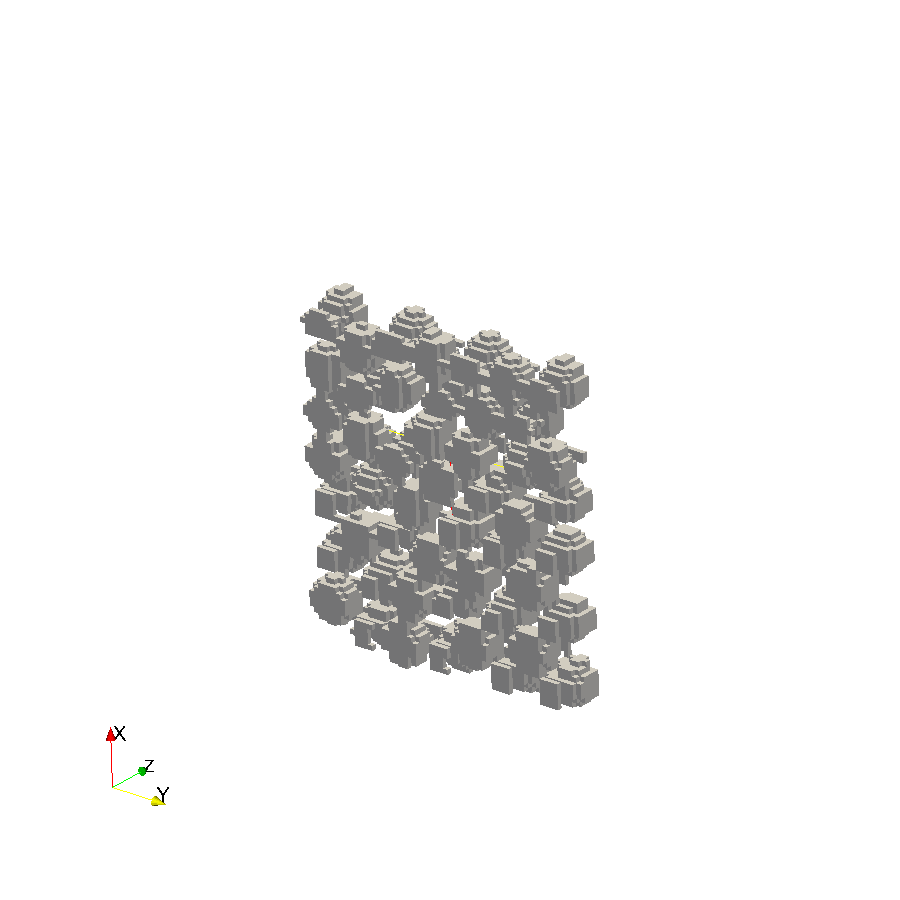
\includegraphics[width=\textwidth, trim={200pt, 150pt, 200pt, 200pt},clip]{figures/lbm/k092res10}
                \caption{Pebble bed with $k = 0.92$, $\res = 10$.}
                \label{fig:k092res10}
        \end{subfigure}%
        ~
        \begin{subfigure}[b]{0.3\textwidth}
                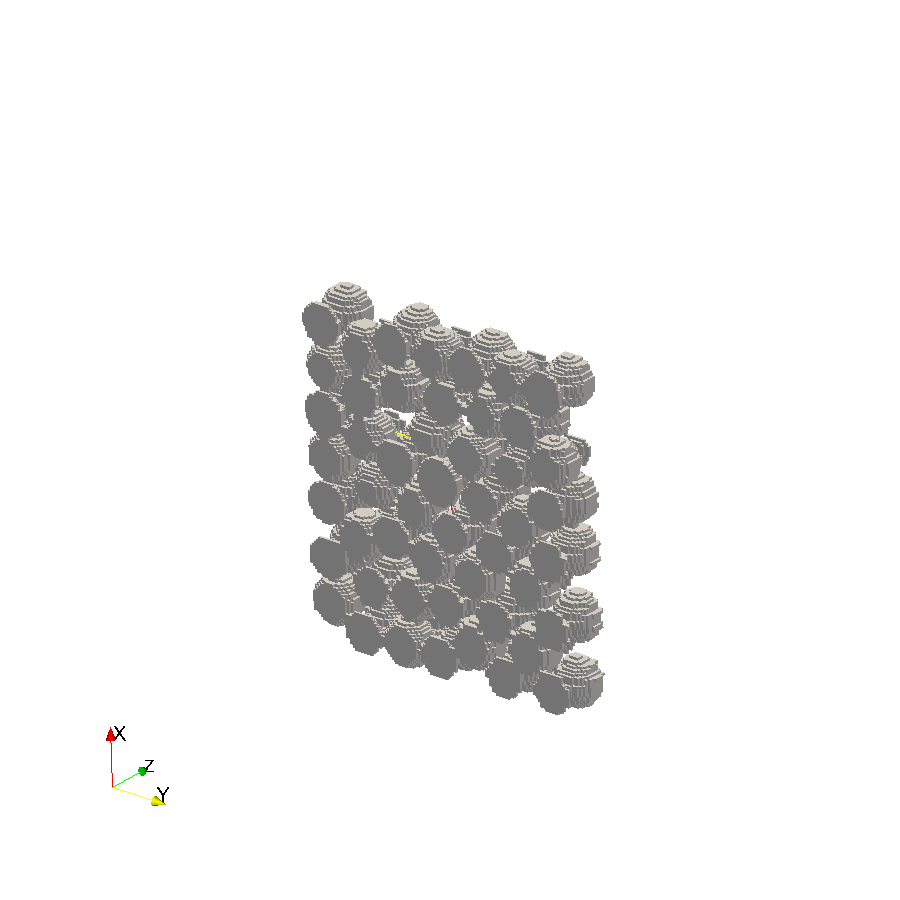
\includegraphics[width=\textwidth, trim={200pt, 150pt, 200pt, 200pt},clip]{figures/lbm/k0947res20}
                \caption{Pebble bed with $k = 0.947$, $\res = 20$.}
                \label{fig:k0947res20}
        \end{subfigure}%
        ~
          %add desired spacing between images, e. g. ~, \quad, \qquad, \hfill etc.
          %(or a blank line to force the subfigure onto a new line)
        \begin{subfigure}[b]{0.3\textwidth}
                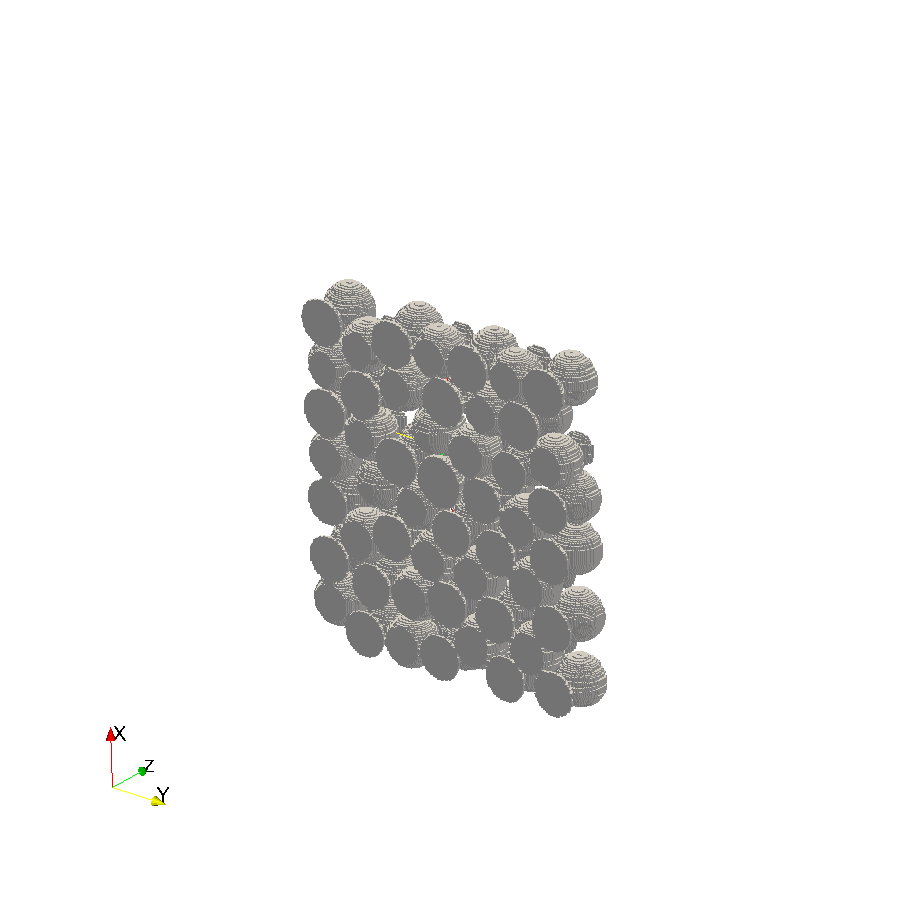
\includegraphics[width=\textwidth, trim={200pt, 150pt, 200pt, 200pt},clip]{figures/lbm/k097res40}
                \caption{Pebble bed with $k = 0.97$, $\res = 40$.}
                \label{fig:k097res40}
        \end{subfigure}
        \caption{For a specified packing fraction, 62.4\%, different resolution lattices require different radius scaling factors. The increased resolution is seen in increasing accuracy of spherical modeling on the discretized lattice.}\label{fig:3d-dem-lbm-mapping}
\end{figure}

When the simplified pebble bed is mapped onto discrete LBM nodes, we see the effects of resolution in \Cref{fig:3d-dem-lbm-mapping}. Here we have chosen resolutions of 10, 20, and 40, respectively. For each resolution, the coarseness of discretization requires varying radius reduction factors in order to achieve a consistent digital packing fraction; k = 0.92, 0.947, and 0.97, respectively. Details of the lattices are given below in \Cref{tab:3d-simp-lbm-parameters}.


\begin{figure}[h]
    \centering
    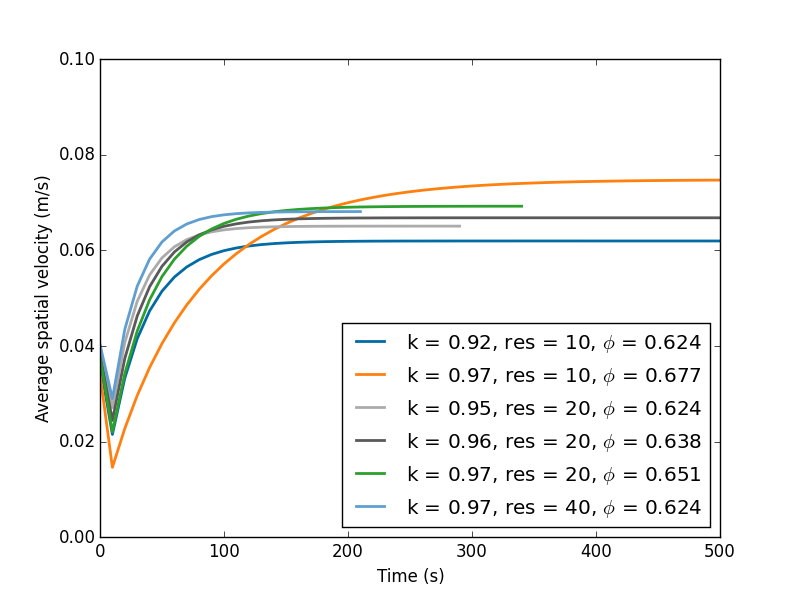
\includegraphics[width=0.75\textwidth]{figures/lbm/3d-lbm-settings-velocity}
    \caption{Averaged system velocity shows pebble beds with the same digital packing fraction and different resolutions will have different average system velocities.}\label{fig:3d-lbm-settings-velocity}
\end{figure}

In \Cref{fig:3d-lbm-settings-velocity}, the lattices shown in \Cref{fig:3d-dem-lbm-mapping} and others have their overall average velocity plotted. In this case, the magnitude of steady-state velocity is important so the integrated velocity has been divided by the total fluid space in the simulation. We see from \Cref{fig:3d-lbm-settings-velocity} that a lattice with the same packing fraction will have slightly different rates at which steady-state is approached. 

\begin{figure}[h]
    \centering
    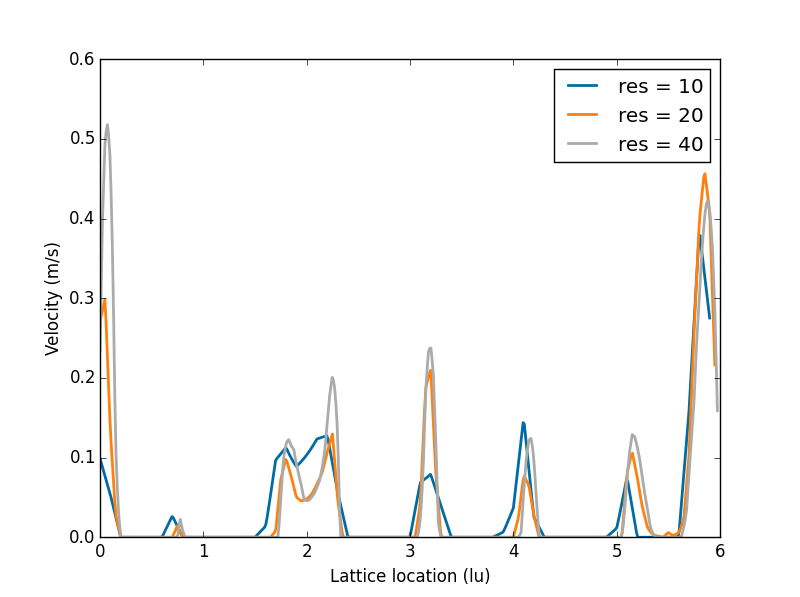
\includegraphics[width=0.5\textwidth]{figures/lbm/3d-bed-v-profiles}
    \caption{Low resolution lattices show qualitatively similar behavior but have insufficient resolution to capture jet velocity magnitudes.}\label{fig:3d-bed-v-profiles}
\end{figure}

At a location along the axial midpoint, velocity profiles across the pebble bed are shown in \Cref{fig:3d-bed-v-profiles}. The velocity jets in the near-wall region, caused by low packing fraction from ordered packing, are not well-captured by the low resolution ($\res = 10$) lattice. Other features of velocity are qualitatively seen in the low resolution packing, such as the velocity near $x = 2$~lu, but the $\res=20$ shows much greater correspondence with the profiles predicted by the highest resolution packing.

\begin{figure}[h]
    \centering
    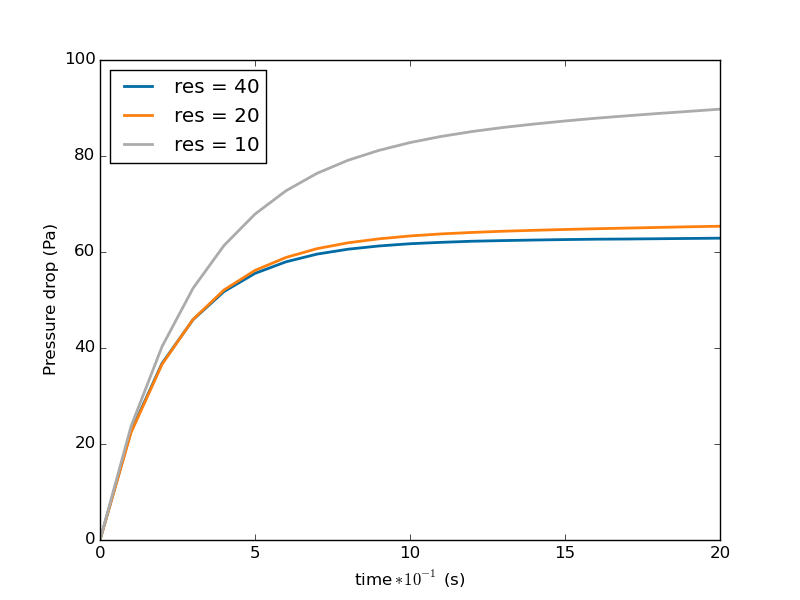
\includegraphics[width=0.5\textwidth]{figures/lbm/3d-study-pressure-drop}
    \caption{Pressure drops across the simplified pebble bed approaching steady-state in time. The low resolution pebble bed greatly over-predicts the pressure drop. Increased resolution appears to converge to approximately \SI{61}{\pascal}.}\label{fig:3d-study-pressure-drop}
\end{figure}

Considerations of the velocity in the packed bed are important because the impact of tortuous velocity pathlines are what we seek to understand with implementation of the DEM-LBM study. However, hydrodynamically, an important measure of the physical fidelity of the packing simulation is the pressure drop across the bed. In \Cref{fig:3d-study-pressure-drop}, the pressure drop between inlet and outlet as a function of time are given for the three packings with equal packing fraction (the beds of \Cref{fig:3d-dem-lbm-mapping}). The pressure drop predicted by the Kozen-Carman relationship is approximately \SI{66}{\pascal}. The steady state value of the $\res=40$ lattice is \SI{61}{\pascal}. The lower resolution, $\res=20$, lattice comes close to the KC prediction; the steady-state pressure drop is \SI{64}{\pascal}. The low resolution pebble bed lattice is unstable and the density blows up shortly after \SI{200}{\sec}.

The last aspect to consider in the execution of the LBM model is the duration of a complete simulation. The last row in \Cref{tab:3d-simp-lbm-parameters} shows the product of total timesteps (to reach 200 s) and total lattice nodes. Assuming a perfect scalability of the simulation, this value is approximately the number of calculations performed to solve for steady-state on the lattice. Normalizing against the $\res=10$ lattice, we see that it requires 16 times longer to run the $\res =20$ lattice and more than 255 times longer to run the $\res = 40$ lattice. The same scaling rules will apply to the full pebble bed lattices that we wish to study. Thus, like most models of packed beds, we are forced to concede some accuracy in physics of the model for simplifications that allow reasonable computational times. For this reason, we conclude that the $\res = 20$ lattice, with $k$ chosen to satisfy digital porosity, is the appropriate setting to continue pebble bed simulations. The $\res = 20$ lattice had reasonable accuracy on hydrodynamic measurements of pressure drop and showed acceptable ability to capture features of the flow velocity such as the near-wall jets.

\begin {table}[h] %
\caption{Comparison of lattice parameters for simplified pebble bed model.}
\label{tab:3d-simp-lbm-parameters} \centering %
\begin{tabular}{@{}lccc@{}}
\toprule %
$\res$   &   10  &   20    &   40  \\\midrule
$N_x$   &   60  &   120 &   240 \\
$N_y$   &   10  &   20  &   40 \\
$N_z$   &   138 &   276 &   553 \\
$N_\text{tot}$  &   \num{82.8e3}     &   \num{662.4e3}    & \num{5308.8e3} \\
$\omega_{ns}$     &   1.131   &   0.789   &   0.491   \\
$\delta_x$  &   0.1     & 0.05  & 0.025 \\
$\delta_t$  & 0.001     &   0.0005  & 0.00025   \\
$N_t$   &   \num{200e3} &    \num{400e3}  & \num{800e3} \\
$N_\text{tot} \times N_t$ & \num{16.6e9} & \num{264.9e9}     & \num{4247.0e9} \\\bottomrule
\end{tabular}
\end{table}




\FloatBarrier

\section{Model Setup \& Methodology}
The purpose of the lattice-Boltzmann simulation is to reveal the influence of tortuous helium flow on energy transport inside the packed bed of a tritium breeder in a fusion reactor. For this reason, we need not study the same parametric space as that of \Cref{sec:isfnt-12}. Instead we can look at the cases of $\phi = 0.64$ initially packed (with no damage) and then $\phi = 0.64$, $r_2^*$, and $\eta = 5\%$, as described thoroughly in \Cref{sec:isfnt-12}. With a resolution of $\res = 20$, the lattice parameters for both beds are given in \Cref{tab:lbm-parameters}. The relaxation parameters, $\omega$, for the lattice solving the momentum equation ($\omega_{ns}$), the lattice nodes representing the solid in the energy equation ($\omega_{cj}$) and the lattice nodes for the fluid in the energy equation ($\omega_{ad}$) are given in \Cref{tab:lbm-relaxations}

% For this lattice-Boltzmann simulation I use a resolution of $\text{res} = 10$ and a time step of $\delta_t = $\num{0.001}. The rest of the descriptions of our pebble bed are locked from the system and material properties. The other geometric values for the lattice are given in Table~\ref{tab:lbm-parameters}, the relaxation parameters defining the collision dynamics of the lattices are given in Table~\ref{tab:lbm-relaxations}, and the boundary conditions are given in Table~\ref{tab:lbm-boundaries}. The values are all unitless in the lattice framework and are translated from the physical values to match the model of pebbles and fluid from \cref{sec:cfd-dem-studies}

\begin {table}[h] %
\caption{Physical description of the lattice (in lattice units).}
\label{tab:lbm-parameters} \centering %
\begin {tabular}{ ccccc }
\toprule %
$N_x$   &   $N_y$  &   $N_z$    &   $\delta_x$   & $\delta_t$    \\\toprule
639      &   200     &   50     &    0.1         &  0.001        \\\bottomrule
\end{tabular}
\end{table}

\begin {table}[h] %
\caption{The momentum relaxation time for fluid (ns), thermal relaxation time for fluid (ad), and thermal relaxation time for the solid (cj) used in the simulation.}
\label{tab:lbm-relaxations} \centering %
\begin {tabular}{ cccccccc }
\toprule %
$\omega_{ns}$ &  $\omega_{ad}$  &   $\omega_{cj}$     \\\toprule
1.131      &  0.788       &   1.365          \\\bottomrule
\end{tabular}
\end{table}

% \begin {table}[htp] %
% \caption{Boundary conditions translated into lattice units.}
% \label{tab:lbm-boundaries} \centering %
% \begin {tabular}{ cccccccc }
% \toprule %
% $\vec{u}_\text{inlet}$    &  $T_\text{inlet}$   &  $T_\text{wall}$     \\\toprule
% (0.005, 0, 0)           &  131.79           &   131.79          \\\bottomrule
% \end{tabular}
% \end{table}


% % The physical properties of helium from \cref{sec:cfd-dem-setup} are used here to calculate the relaxation time, $\tau_{ns}$ as outlined in \cref{sec:physical-to-lattice}. The physical description of the pebble bed analyzed with LBM is identical to the beds described in \cref{sec:cfd-dem-studies}. The details for mapping from our DEM packing to the LBM lattice are given in \cref{sec:dem2lbm-mapping}. With the mechanisms described there we can define the lattice nodes definitions (being either solid or fluid) simply with specifying the resolution.

% The relaxation parameter describing the collisions of density distribution functions on the Navier-Stokes lattice (NS-lattice) allowed for achieving a stable and steady fluid velocity. Unfortunately, from the physical properties of ceramic pebbles and thermal properties of helium, the relaxation times on the thermal lattices would only allow the simulation to run until instabilities at the outlet propagates upstream and destroys the results of the entire thermal lattice. These preliminary results will therefore focus on the velocity results and the initial thermal results (it would not reach thermal steady-state before crashing). Even with this caveat on the results, what we do see from the LBM results are extremely encouraging for the use of the method in the future.






% \section{Laminar Mixing of Energy in Packed Beds with Volumetric Heating}

% In the plot of \Cref{fig:lbm-streamlines}, streamlines are created along the $y$-direction at the inlet. The streamlines show the inlet helium moving in a tortuous path as it winds through the pebble bed and picks up the energy which has been deposited into the pebbles from a volumetric heat source. The complete tortuous flow field solved in the LBM computations reveals an extremely important feature of the helium purge gas that has, up to now, not been realized.

% Moving up through the $x$ direction of the pebble bed (the direction of the mean flow), several temperature profiles of the fluid and solid are shown in \Cref{fig:lbm-temp-profiles}. The temperature profiles all demonstrate a profile that does not match predicted profiles through pebble beds when constant $\keff$ models are applied to the bed in its continuum treatment. For comparison, the dashed line in \Cref{fig:lbm-temp-profiles} is a parabolic curve with match $\Delta T$ to the profile from $x^* = 10$. 

% Let us explore further the deviation from a parabolic fit and the consequences on solid breeder design that appear from the LBM simulations. In the experimental quantifications of heat transport in pebble beds with interstitial helium, conduction is the only mode of heat transfer considered. The Grashoff number inside a packed bed is small enough that any natural convection cells will most certainly be negligible to heat transfer compared to the conduction through the fluid. Thus, experimentalists can describe the effective thermal conductivity of the combination of solid and gas. These are the values reported in, \textit{e.g.}, \Cref{fig:keff}. The DEM and CFD-DEM studies seemed to support these models as temperature profiles emerged from those simulations that fit nearly perfectly to parabolic profiles of varying $\keff$. Going the other way, if you had a constant $\keff$ of a pebble bed with helium, you could predict temperature profiles, and importantly maximum temperatures, in the solid breeder volume. 

% The $\keff$ value represents the rate at which the solid breeder volume can move energy into the cooling structure. When a perfect parabolic temperature profile is found (such as in the DEM and CFD-DEM results) the $\keff$ is calculated simply from the input volumetric heat source and the $\Delta T$ between centerline and wall. However, because the results from LBM do not fit into a perfect parabolic profile, I fit a parabola of a constant $\keff$ model to the \textit{amount of energy in the profile}. In other words, I integrate the temperature profile from LBM along the $y$ length and find a parabolic profile which, when integrated along the same direction, yields the same value,
% \begin{equation}
%     \int_0^{Y^*} T_{lbm}(y)\,\mathrm{d}y = \int_0^{Y^*} (1-y^2)T_{cl} + T_w y^2
% \end{equation}
% where $T_w$ is the constant temperature wall boundary condition and $T_{cl}$ is the centerline temperature. An iterative procedure is run through until a correct $T_{cl}$ is found which satisfies the equality. When this procedure is carried out, I find the parabola shown in \Cref{fig:lbm-temp-parabolas}.

% Reiterating, the parabola of \Cref{fig:lbm-temp-parabolas} is the shape of temperature profile at which the same amount of energy is removed from the system in a constant $\keff$ condition as is removed from the actual LBM result. What we see in the figure is the LBM result is showing a lower maximum temperature and higher temperature near the walls. This shows that for the amount of energy removed from a pebble bed with flowing helium, the maximum temperature is lower than what would be predicted from current models!

% The phenomena of the flowing helium lowering the maximum temperature in the centerline of the bed and raising the temperature on the edges is something I have given the name of \textit{laminar mixing of energy}. The low Reynolds number flow of helium remains laminar and thus energy transport perpendicular to the flow path of the fluid is still pure conduction. But the tortuous path of helium as it snakes through the pebble bed mixes the energy of hot pebbles in the center and comparatively cooler pebbles near the walls.

% % It is well known that a fluid moving through a packed bed will follow a path much longer than the length of the packed bed. The extended path is often reported as the tortuosity of the packed bed. In the ceramic breeder packed beds for tritium generation, the tortuosity of the helium flow modeled in LB resulted in 

% % \begin{figure}[t]
% %     \centering
% %     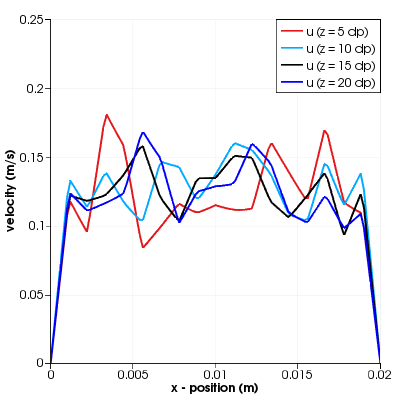
\includegraphics[width=\singleimagewidth]{figures/lbm/evap-u-profiles}
% %     \caption{Velocity profiles (in the $x$-direction) at varying pebble bed heights for the pebble bed with 10\% damaged pebbles.}\label{fig:lbm-evap-u-profile}
% % \end{figure}

% \begin{figure}[t]
%     \centering
%     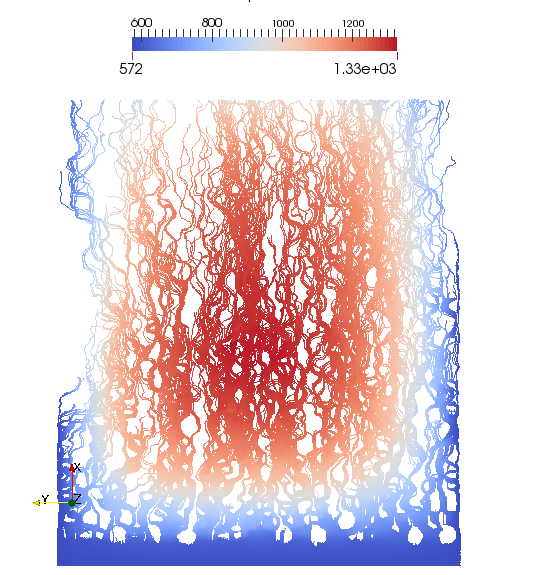
\includegraphics[width=\singleimagewidth]{figures/lbm/lbm-streamlines}
%     \caption{Demonstrating the meandering path -- importantly wandering in the $x$-direction -- of fluid flow in the pebble bed.}\label{fig:lbm-streamlines}
% \end{figure}

% \begin{figure}[t]
%     \centering
%     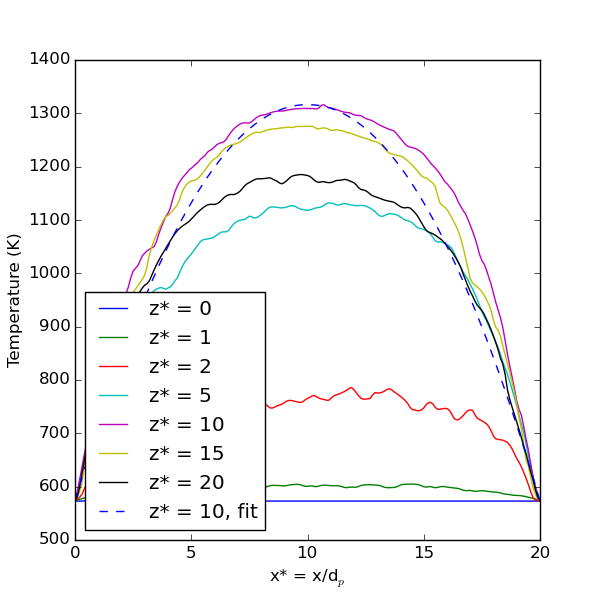
\includegraphics[width=\singleimagewidth]{figures/lbm/lbm-temp-profiles}
%     \caption{Temperature profiles (in the $x$-direction) at varying pebble bed heights for the pebble bed with 10\% damaged pebbles. Shown for comparison is a parabolic profile that had fit both DEM and CFD-DEM temperature results.}\label{fig:lbm-temp-profiles}
% \end{figure}

% \begin{figure}[t]
%     \centering
%     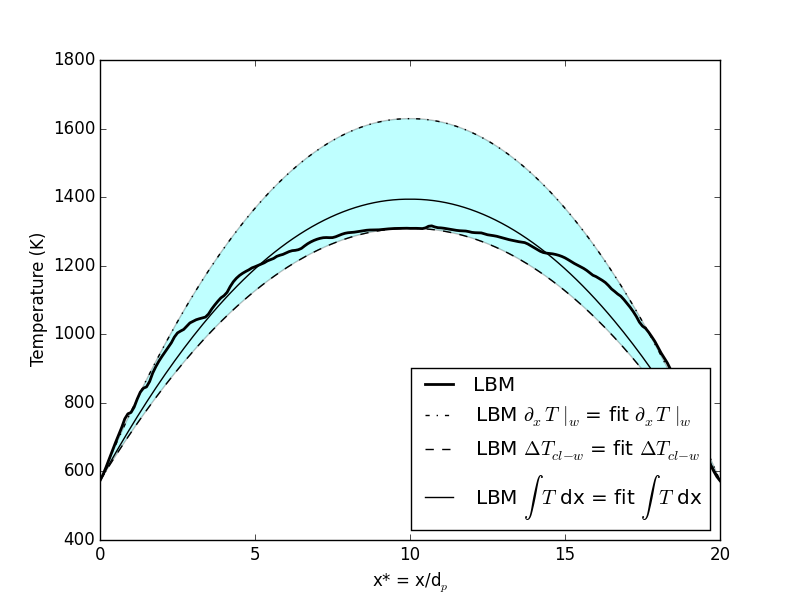
\includegraphics[width=\singleimagewidth]{figures/lbm/lbm-temp-profile_parabolic}
%     \caption{A parabolic fit to the integrated energy of a temperature profile compares to the temperature profile from LBM. The LBM temperature profile increases near the walls and is flattened near the centerline. The behavior is indicative of laminar mixing of energy in the bed.}\label{fig:lbm-temp-parabolas}
% \end{figure}

% \begin{figure}[t]
%     \centering
%     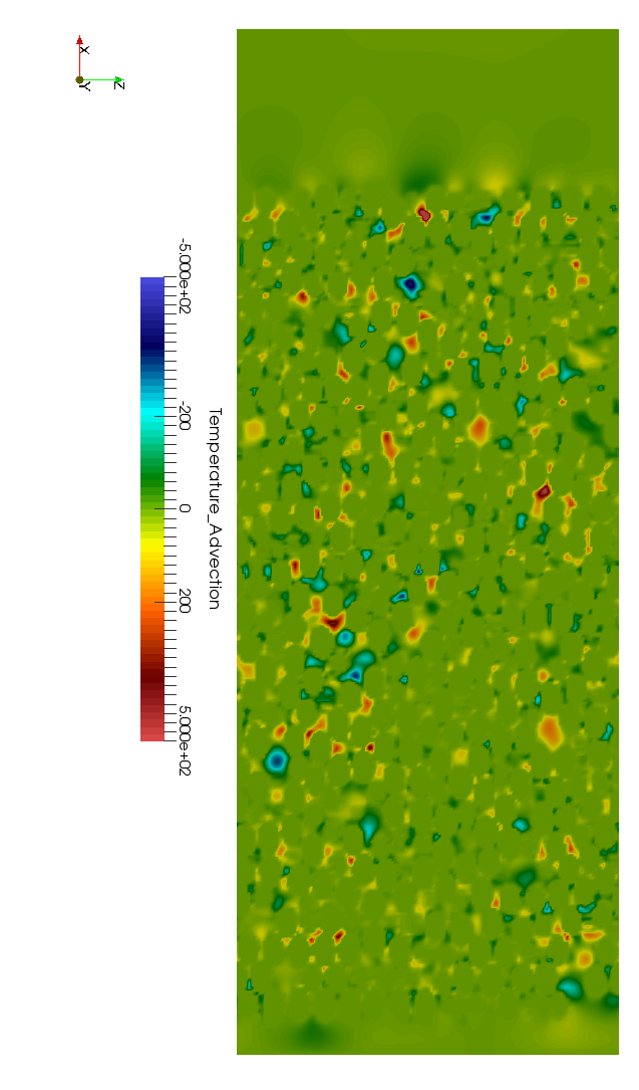
\includegraphics[width=\singleimagewidth]{figures/lbm/lbm-laminar-mixing}
%     \caption{Mean flow direction is in the positive $x$ direction. This $x$-$z$-plane slice shows the $y$ components of velocity as the fluid moves into/out of the plane - mixing the energy with laminar flow.}\label{fig:lbm-laminar-mixing}
% \end{figure}

% \FloatBarrier
% \section{Conclusions}




